In this section, we discuss our approach for the large-scale detection of drive-by downloads and how we want to implement it in a proof of concept. But we start with investigating how to correlate different HTTP requests that logically belong together.

\subsection{Correlating HTTP requests}
\label{sigh}

The challenge faced when multiple websites have to be loaded at the same time, is to know which HTTP request corresponds to which website. Many webpages consist of dozens of resources that have to be loaded. The loading of some resources can even be delayed until after certain predefined events. In some libraries, the requesting of a web resource consists of several independent steps.

An easy solution would be to modify the web browser in such a way that it exposes this information with an easy to use interface. While this would solve the problem, regular maintenance would be required to keep this system working. 

A solution could be to log all the network traffic and analyse it. While this information is always available, it would require complex protocol and content parsers to reconstruct the original network streams and extract useful information from it. Additionally, an encrypted connection would require a proxy that uses on-the-fly creation of certificates. Even then it would be trivial to circumvent this system as scripting languages and browser plug-ins could be used to dynamically request resources.

% \thispagestyle{empty}
\begin{figure}[h]
    \centering
    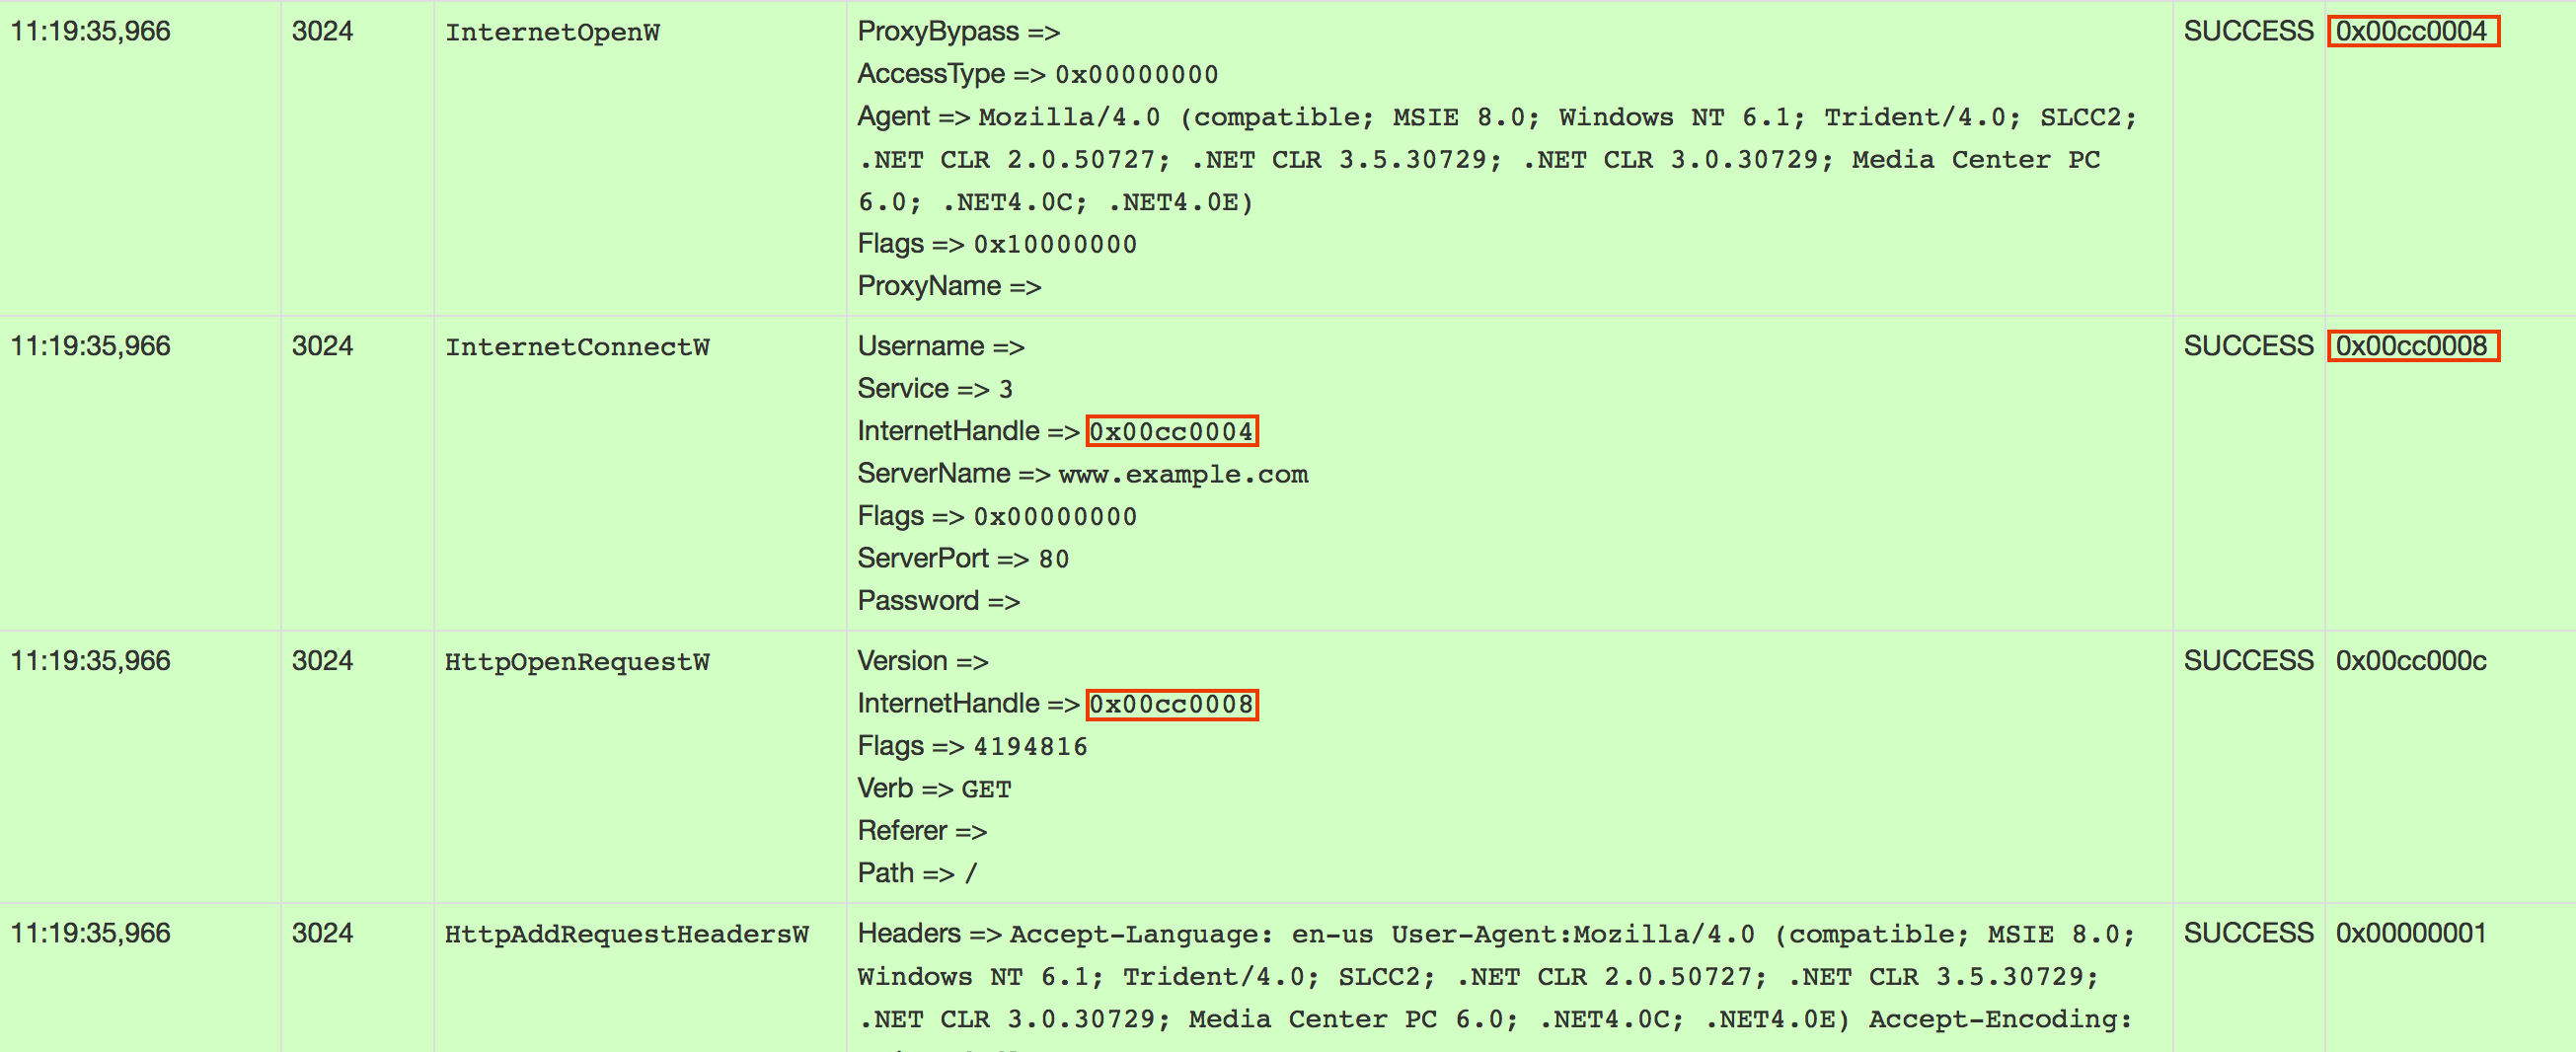
\includegraphics[width=14.7cm]{Images/wininet.png}
    \caption{Example of the API calls involved when the WinINet library is used to load a URL. The red rectangles show the handles that can be used to identify the API calls that belong to a single request.}
    \label{fig:wininet}
\end{figure}
% \restoregeometry

A better solution would be to correlate an HTTP request to its originating webpage by observing the behaviour and environment of the web browser. By hooking and logging the API calls that are made by the web browser, the full process and thread context of every call is available or can be reconstructed from earlier calls (as can be seen in figure \ref{fig:wininet}). As all modern web browsers use high-level network libraries, this is the ideal place to monitor. When combined with other interesting APIs, a full insight in the behaviour of the web browser is available and detecting malicious behaviour is a matter of writing the correct behavioural analysers.

An alternative for API hooking would be to write a custom operating system driver and monitor the syscalls. While this would still give most of the information API hooking would give and much harder to detect by the malware, it is much harder to implement and the information gained from intercepting the API calls to the high-level network libraries would not be available.

\subsection{Algorithm}
\begin{figure}[h]
    \centering
    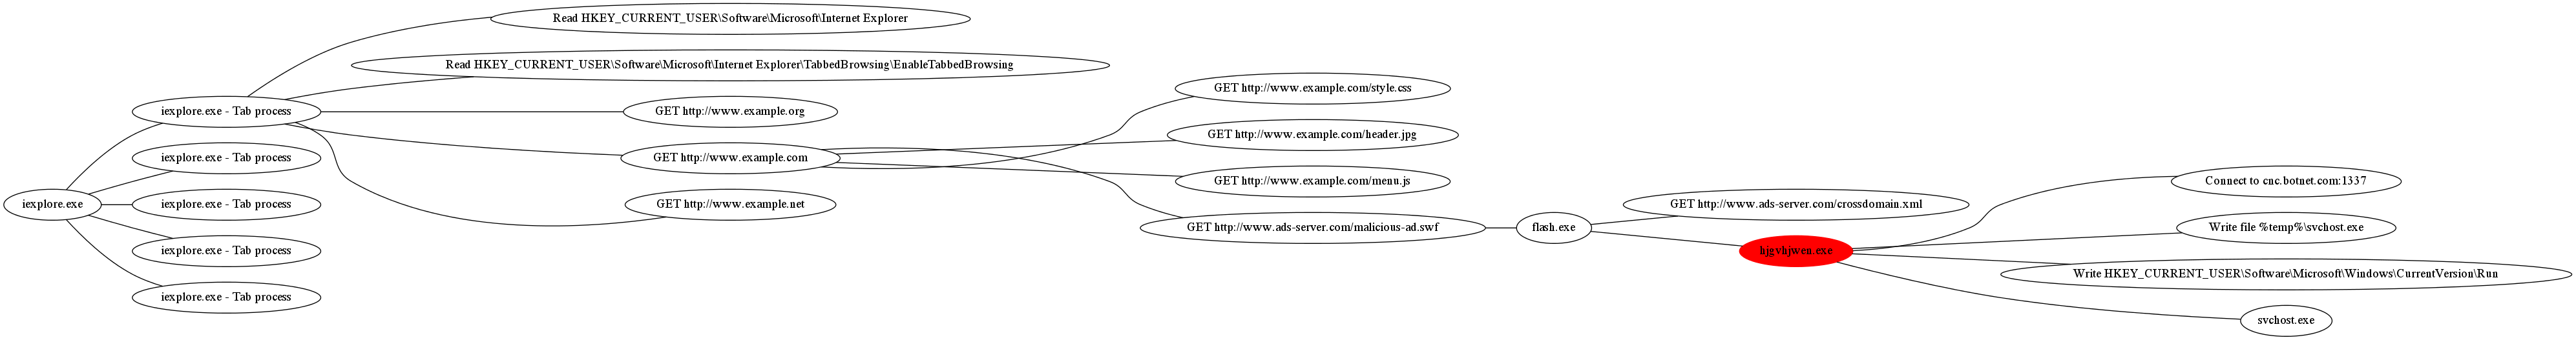
\includegraphics[width=17cm]{Images/alg_tree.png}
    \caption{An example of the graph}
    \label{fig:alg_tree}
\end{figure}

\subsubsection{Design considerations}

\subsubsection{Generic algorithm}

- Disconnected DAGs

1) Hooker schrijven voor elke browser die trafiek tussen Netwerk en Browser of in de browser zelf monitort en doorgeeft aan Cuckoo
2) DAG opstellen door de extra informatie te gebruiken in report.json
3) DAG interpreteren, nodes met enkel uitgaande edges zijn de beginnende URL
4) Kijken of er iets raar gebeurt in elk eiland
5) Reporting

\subsubsection{Platform-specific challenges}

Unix heeft geen handles zoals Windows maar meer files
	- FD's eigenlijk

\subsubsection{Alternative approaches}

- pcap / mitm
- tijd based
- aangepaste headers

\subsection{Proof of Concept}
\epigraph{You're the chosen one, Cuckoo.}{Adriaan}

\textbf{TOEKOMSTIGE TIJD}

For the Proof of Concept (PoC), Cuckoo \cite{cuckoo} will be used. Cuckoo is a malware analysis system that runs malware in a virtual environment, tracks its behavior and reports these results to the user.\\

Cuckoo was choosen because it already implements a great deal of the prerequisites of the algorithm, discussed in \todo{add ref}. Cuckoo, through Cuckoomon \cite{cuckoomon}, provides a series of hooks which monitors calls between the browser and the operating system. This allows us to monitor the extra information from section \ref{algo2}. 

These hooks, conveniently, also monitor the network calls made by the browser. Although only Internet Explorer is supported by Cuckoo, due to the scope of the project, this is not a problem.

\subsubsection{Prerequisites and changes}

Internet Explorer uses Windows' ``Secure Channel'' or ``Schannel'' \cite{schannel} to encrypt HTTP requests and decrypt HTTP responses. This will allow us to monitor traffic on the operating system level without any need for a proxy to decrypt the traffic.

As already explained, Cuckoo uses Cuckoomon, which uses hooks to monitor calls, to keep track of the browser activity. Besides adding a few new hooks and deleting a few irrelevant hooks for drive-by downloads, nothing major has to be changed to Cuckoomon.\todo{Uitleggen welke hooks precies?}

The current development version, \texttt{1.2-dev},  only accepts one URL at a time. To allow for concurrently visiting multiple websites in one sandbox environment, Cuckoo has to be extended.

\subsubsection{The Setup}

To test the algorithm, we will use the adapted Cuckoo with Virtualbox as the sandbox environment. As the virtual machine's operating system, we will use Windows 7 as this is still the operating system which is most targeted by malware. As the browser, we will use Internet Explorer 8 to actually allow the malware to successfully perform the drive-by download.

The virtual machine will be provisioned with the Top 20 of visited websites in the Netherlands, according to Alexa \cite{http://www.alexa.com/topsites/countries/NL}, and with current malware floating on the internet.\todo{Mss toch niet zeggen?}

The structure of the graph will be tree-like, as suggested in \todo{ref naar algo}. Figure \ref{fig:alg_tree}.

Figure \ref{fig:alg_tree} also shows a website with a drive-by download. In the top left, one can see process spawns (red vertices) in an unusual place.\todo{beter uitleggen}

\begin{figure}[h]
    \centering
    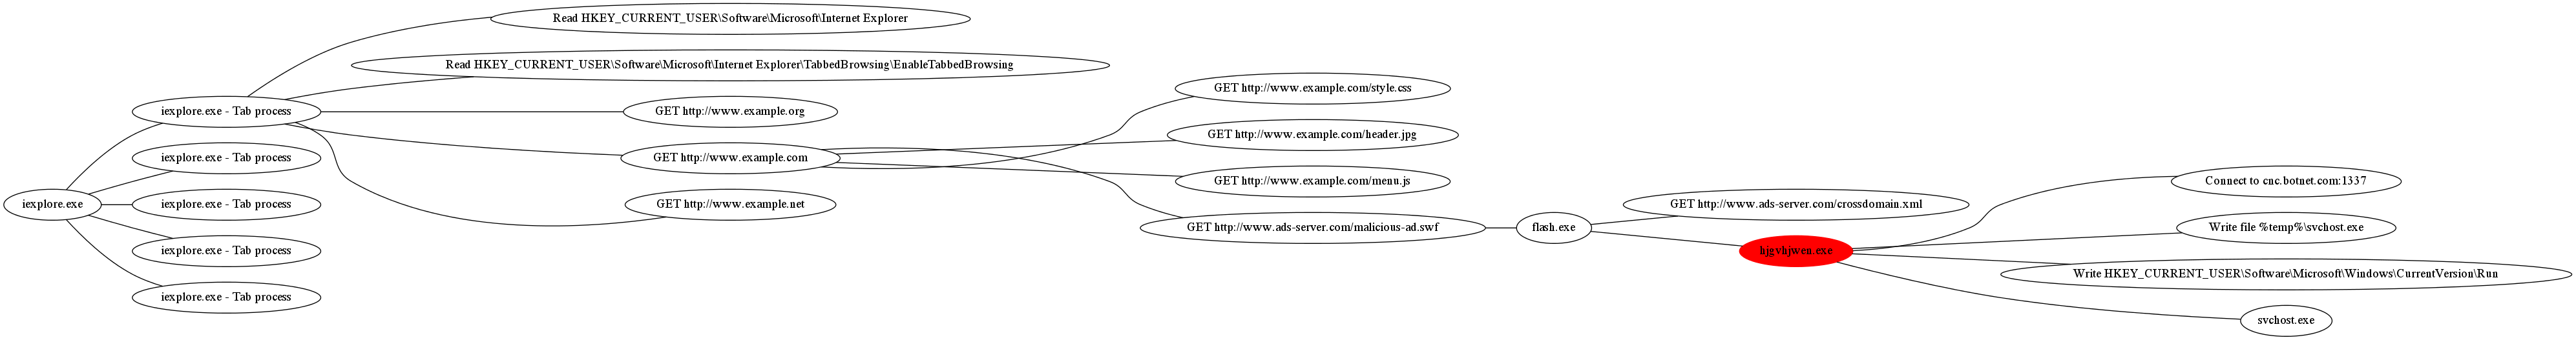
\includegraphics[width=17cm]{Images/alg_tree.png}
    \caption{An example of the graph}
    \label{fig:graph}
\end{figure}


